\documentclass[12pt]{article}

% Source text: Tutorial-3.pdf 
% Style reference: MH5200_ProblemSheet2.tex 

\usepackage[margin=1in]{geometry}
\usepackage{amsmath,amssymb,mathtools}
\usepackage{enumitem}
\usepackage{bm}
\usepackage{hyperref}
\usepackage{fancyhdr}
\usepackage{draftwatermark}
\usepackage{xcolor}
\usepackage{pgfplots}
%------------- TITLE AND METADATA -------------

\newcommand{\CourseCode}{MH1101 }
\newcommand{\CourseName}{Calculus II}
\newcommand{\DocType}{Tutorial 3 (Week 4) -- Problems \& Solutions}

\title{
\CourseCode \CourseName \\[0.3em]
\large \DocType
}
\author{
  Academic Year 2025/2026, Semester 2 \\[0.25em]
  \textit{Quantitative Research Society @NTU}
}
\date{\today}

%------------- HEADER & FOOTER (for page 2 onward) -------------
\fancypagestyle{main}{
  \fancyhf{}
  \fancyhead[L]{\CourseCode \CourseName}
  \fancyhead[R]{\href{https://qrsntu.org}{QRS@NTU}}
  \fancyfoot[C]{\thepage}
  \renewcommand{\headrulewidth}{0.4pt}
  \renewcommand{\footrulewidth}{0pt}
}

%------------- SIMPLE FOOTER (page 1 only) -------------
\fancypagestyle{plainfirst}{
  \fancyhf{}
  \renewcommand{\headrulewidth}{0pt}
  \renewcommand{\footrulewidth}{0pt}
  \fancyfoot[C]{\scriptsize\textcolor{gray}{\textit{For academic reference only. This document is provided for educational purposes and does not constitute an official question paper, answer key, or any formally authorised academic material. Its content is not guaranteed to be complete or accurate.}}}
}

%------------- WATERMARK -------------
\SetWatermarkText{Unofficial — QRS@NTU — qrsntu.org}
\SetWatermarkScale{1}
\SetWatermarkLightness{0.99}

\begin{document}

%------------- COVER PAGE -------------
\maketitle
\thispagestyle{plainfirst}
\pagestyle{main}

\bigskip

%====================================================
% OVERVIEW
%====================================================

\begin{center}
\rule{0.8\textwidth}{0.4pt}\\[4pt]
\textbf{Overview} \\[2pt]
\rule{0.8\textwidth}{0.4pt}
\end{center}

\noindent
This tutorial focuses on core techniques for improper integrals and on geometric applications of integration.

\begin{itemize}[leftmargin=*]
\item Improper integrals: convergence tests and evaluation by limits.
\item A basic invariance property of convergent two-sided improper integrals.
\item Areas between curves via intersection analysis and definite integrals.
\item Volumes of revolution using the disk-washer method (and cross-checks via shells).
\item Cylindrical shells: when and why shells are more convenient than washers.
\end{itemize}

\bigskip

\newpage

%====================================================
% QUESTION 1
%====================================================

\section*{Question 1 (Improper integrals)}

\subsection*{Problem}
Determine whether each integral is convergent or divergent. Evaluate those that are convergent.
\begin{enumerate}[label=(\alph*)]
\item \(\displaystyle \int_{-\infty}^{0} \frac{1}{3-4x}\,dx\).
\item \(\displaystyle \int_{e}^{\infty} \frac{1}{x(\ln x)^3}\,dx\).
\item \(\displaystyle \int_{-\infty}^{\infty} (x^3-3x^2)\,dx\).
\item \(\displaystyle \int_{-\infty}^{\infty} x e^{-x^2}\,dx\).
\item \(\displaystyle \int_{-2}^{3} \frac{1}{x^4}\,dx\).
\end{enumerate}

\subsection*{Solution}

\subsubsection*{Method 1: Direct limit evaluation (antiderivatives + improper limits)}

\begin{enumerate}[label=(\alph*)]
\item Consider
\[
\int_{-\infty}^{0}\frac{1}{3-4x}\,dx
=
\lim_{b\to -\infty}\int_{b}^{0}\frac{1}{3-4x}\,dx.
\]
An antiderivative is
\[
\int \frac{1}{3-4x}\,dx = -\frac14 \ln|3-4x| + C.
\]
Hence
\begin{align*}
\int_{b}^{0}\frac{1}{3-4x}\,dx
&=
-\frac14\ln|3|
+\frac14\ln|3-4b|\\
&=\frac14\ln\!\Big(\frac{3-4b}{3}\Big).
\end{align*}
As \(b\to-\infty\), \(3-4b\to\infty\), so the above tends to \(+\infty\). Therefore
\[
\boxed{\text{Divergent (diverges to }+\infty\text{).}}
\]

\item Consider
\[
\int_{e}^{\infty} \frac{1}{x(\ln x)^3}\,dx
=
\lim_{B\to\infty}\int_{e}^{B} \frac{1}{x(\ln x)^3}\,dx.
\]
Use \(u=\ln x\), so \(du=\frac{1}{x}dx\). When \(x=e\), \(u=1\); when \(x=B\), \(u=\ln B\). Thus
\begin{align*}
\int_{e}^{B} \frac{1}{x(\ln x)^3}\,dx
&= \int_{1}^{\ln B} u^{-3}\,du
= \left[-\frac{1}{2u^{2}}\right]_{1}^{\ln B}\\
&= -\frac{1}{2(\ln B)^2}+\frac12.
\end{align*}
Letting \(B\to\infty\) gives \(-\frac{1}{2(\ln B)^2}\to 0\). Hence
\[
\boxed{\text{Convergent, and } \displaystyle \int_{e}^{\infty} \frac{1}{x(\ln x)^3}\,dx=\frac12.}
\]

\item A two-sided improper integral satisfies
\[
\int_{-\infty}^{\infty} (x^3-3x^2)\,dx
=
\int_{-\infty}^{0}(x^3-3x^2)\,dx
+
\int_{0}^{\infty}(x^3-3x^2)\,dx
\]
provided both one-sided integrals converge. But
\[
\int_{0}^{\infty} (x^3-3x^2)\,dx
=
\lim_{B\to\infty}\left[\frac{x^4}{4}-x^3\right]_{0}^{B}
=
\lim_{B\to\infty}\left(\frac{B^4}{4}-B^3\right)=+\infty,
\]
so the integral diverges. Therefore
\[
\boxed{\text{Divergent.}}
\]

\item Compute
\[
\int_{-\infty}^{\infty} x e^{-x^2}\,dx
=
\lim_{A\to\infty}\int_{-A}^{A} x e^{-x^2}\,dx.
\]
Use the antiderivative \(\int x e^{-x^2}dx=-\tfrac12 e^{-x^2}+C\). Then
\[
\int_{-A}^{A} x e^{-x^2}\,dx
=
\left[-\frac12 e^{-x^2}\right]_{-A}^{A}
=
-\frac12 e^{-A^2} + \frac12 e^{-A^2} = 0.
\]
Taking \(A\to\infty\) yields
\[
\boxed{\text{Convergent, and } \displaystyle \int_{-\infty}^{\infty} x e^{-x^2}\,dx = 0.}
\]

\item Since \(x=0\) is a singularity in \([-2,3]\), the integral is improper:
\[
\int_{-2}^{3}\frac{1}{x^4}\,dx
=
\int_{-2}^{0}\frac{1}{x^4}\,dx + \int_{0}^{3}\frac{1}{x^4}\,dx,
\]
if both integrals converge.
Consider
\[
\int_{0}^{3}\frac{1}{x^4}\,dx
=
\lim_{\varepsilon\downarrow 0}\int_{\varepsilon}^{3} x^{-4}\,dx
=
\lim_{\varepsilon\downarrow 0}\left[-\frac{1}{3x^3}\right]_{\varepsilon}^{3}
=
\lim_{\varepsilon\downarrow 0}\left(-\frac{1}{81}+\frac{1}{3\varepsilon^3}\right)=+\infty.
\]
Thus
\[
\boxed{\text{Divergent.}}
\]
\end{enumerate}

\subsubsection*{Method 2: Convergence tests and structure (comparison, \(p\)-test, symmetry)}

\begin{enumerate}[label=(\alph*)]
\item As \(x\to-\infty\), \(\frac{1}{3-4x}\sim \frac{1}{-4x}\), and
\(\int_{-\infty}^{-1}\frac{1}{|x|}\,dx\) diverges, so by comparison the integral diverges.

\item With \(u=\ln x\), the integral becomes \(\int_{1}^{\infty} u^{-3}\,du\), which converges by the \(p\)-test (\(p=3>1\)), and evaluates to \(\frac12\).

\item Polynomials do not decay at infinity: since \(x^3-3x^2 \ge \frac12 x^3\) for all sufficiently large \(x\), and \(\int^{\infty} x^3\,dx\) diverges, the integral diverges.

\item The integrand \(x e^{-x^2}\) is an odd function, so for every \(A>0\),
\(\int_{-A}^{A} x e^{-x^2}\,dx=0\); moreover, the tails decay rapidly, so the improper integral converges and equals \(0\).

\item Near \(x=0\), \(\frac{1}{x^4}\) behaves like a \(p\)-integral with \(p=4\ge 1\), hence \(\int_{0}^{1}x^{-4}\,dx\) diverges, so the given integral diverges.
\end{enumerate}

\newpage

%====================================================
% QUESTION 2
%====================================================

\section*{Question 2 (Two-sided improper integrals)}

\subsection*{Problem}
Suppose both \(\displaystyle \int_{-\infty}^{c} f(x)\,dx\) and \(\displaystyle \int_{c}^{\infty} f(x)\,dx\) are convergent for any real number \(c\). Show that for any real number \(a\) and \(b\),
\[
\int_{-\infty}^{a} f(x)\,dx + \int_{a}^{\infty} f(x)\,dx
=
\int_{-\infty}^{b} f(x)\,dx + \int_{b}^{\infty} f(x)\,dx.
\]

\subsection*{Solution}

\subsubsection*{Method 1: Additivity and cancellation on finite intervals}

Assume first \(a<b\) (the case \(b<a\) is analogous). Since all the displayed improper integrals converge by hypothesis, finite-interval additivity applies:
\[
\int_{-\infty}^{b} f(x)\,dx
=
\int_{-\infty}^{a} f(x)\,dx + \int_{a}^{b} f(x)\,dx,
\]
and similarly
\[
\int_{a}^{\infty} f(x)\,dx
=
\int_{a}^{b} f(x)\,dx + \int_{b}^{\infty} f(x)\,dx.
\]
Rearrange the second identity to get
\[
\int_{b}^{\infty} f(x)\,dx
=
\int_{a}^{\infty} f(x)\,dx - \int_{a}^{b} f(x)\,dx.
\]
Now add the two expressions for \(\int_{-\infty}^{b} f\) and \(\int_{b}^{\infty} f\):
\begin{align*}
\int_{-\infty}^{b} f(x)\,dx + \int_{b}^{\infty} f(x)\,dx
&=
\left(\int_{-\infty}^{a} f(x)\,dx + \int_{a}^{b} f(x)\,dx\right)
+
\left(\int_{a}^{\infty} f(x)\,dx - \int_{a}^{b} f(x)\,dx\right)\\
&=
\int_{-\infty}^{a} f(x)\,dx + \int_{a}^{\infty} f(x)\,dx.
\end{align*}
This proves the desired equality.

\subsubsection*{Method 2: Truncation to \([-M,N]\) and independence of the split point}

Fix any real \(c\) and define
\[
I(c) := \int_{-\infty}^{c} f(x)\,dx + \int_{c}^{\infty} f(x)\,dx.
\]
For \(M,N>0\), consider the finite integral
\[
I_{M,N} := \int_{-M}^{N} f(x)\,dx.
\]
For any split point \(c\),
\[
\int_{-M}^{N} f(x)\,dx
=
\int_{-M}^{c} f(x)\,dx + \int_{c}^{N} f(x)\,dx.
\]
Now take limits \(M\to\infty\) and \(N\to\infty\). The hypothesis implies both \(\int_{-\infty}^{c} f\) and \(\int_{c}^{\infty} f\) exist, and hence
\[
\lim_{M\to\infty}\int_{-M}^{c} f(x)\,dx = \int_{-\infty}^{c} f(x)\,dx,\qquad
\lim_{N\to\infty}\int_{c}^{N} f(x)\,dx = \int_{c}^{\infty} f(x)\,dx.
\]
Therefore,
\[
\lim_{M,N\to\infty} I_{M,N}
=
I(c).
\]
The left-hand side does not depend on \(c\), so \(I(c)\) is constant in \(c\). In particular \(I(a)=I(b)\), which is exactly the required identity.

\newpage

%====================================================
% QUESTION 3
%====================================================

\section*{Question 3 (Areas between curves)}

\subsection*{Problem}
Sketch the region enclosed by the given curves, and find its area.
\begin{enumerate}[label=(\alph*)]
\item \(y = \sqrt{x+3}\), \(y = \dfrac{x+3}{2}\).
\item \(4x + y^2 = 12\), \(x = y\).
\item \(y = \cos x\), \(y = \sin 2x\), \(x=0\), \(x=\dfrac{\pi}{2}\).
\end{enumerate}

\subsection*{Solution}

\subsubsection*{Method 1: Standard ``top-minus-bottom'' / ``right-minus-left'' integrals}

\begin{enumerate}[label=(\alph*)]
\item Intersections satisfy \(\sqrt{x+3}=\frac{x+3}{2}\). Let \(u=x+3\ge 0\). Then \(\sqrt{u}=\frac{u}{2}\) gives \(u=0\) or \(u=4\), hence \(x=-3\) or \(x=1\).
On \([-3,1]\), \(\sqrt{x+3}\ge \frac{x+3}{2}\). The area is
\begin{align*}
A
&=\int_{-3}^{1}\left(\sqrt{x+3}-\frac{x+3}{2}\right)\,dx
=\int_{0}^{4}\left(\sqrt{u}-\frac{u}{2}\right)\,du\\
&=\left[\frac{2}{3}u^{3/2}-\frac{u^2}{4}\right]_{0}^{4}
=\frac{16}{3}-4=\frac{4}{3}.
\end{align*}
\[
\boxed{A=\frac{4}{3}.}
\]

\item Write the parabola as \(x = 3-\frac{y^2}{4}\). The line is \(x=y\).
Their intersections satisfy \(y=3-\frac{y^2}{4}\), i.e.
\(y^2+4y-12=0\), so \(y=2\) or \(y=-6\).
On \([-6,2]\), the parabola lies to the right of the line. Hence
\begin{align*}
A
&=\int_{-6}^{2}\left(\left(3-\frac{y^2}{4}\right)-y\right)\,dy
=\int_{-6}^{2}\left(3-y-\frac{y^2}{4}\right)\,dy\\
&=\left[3y-\frac{y^2}{2}-\frac{y^3}{12}\right]_{-6}^{2}
=\frac{10}{3}-(-18)=\frac{64}{3}.
\end{align*}
\[
\boxed{A=\frac{64}{3}.}
\]

\item Solve \(\cos x=\sin 2x\) on \([0,\frac{\pi}{2}]\):
\[
\cos x = 2\sin x\cos x \quad\Rightarrow\quad
\cos x=0 \text{ or } \sin x=\frac12,
\]
so \(x=\frac{\pi}{2}\) or \(x=\frac{\pi}{6}\).
On \([0,\frac{\pi}{6}]\), \(\cos x \ge \sin 2x\); on \([\frac{\pi}{6},\frac{\pi}{2}]\), \(\sin 2x \ge \cos x\).
Thus
\begin{align*}
A
&=\int_{0}^{\pi/6}(\cos x-\sin 2x)\,dx
+\int_{\pi/6}^{\pi/2}(\sin 2x-\cos x)\,dx\\
&=\left[\sin x+\frac12\cos 2x\right]_{0}^{\pi/6}
+\left[-\frac12\cos 2x-\sin x\right]_{\pi/6}^{\pi/2}\\
&=\left(\frac12+\frac14-\frac12\right)+\left(\left(\frac12-1\right)-\left(-\frac14-\frac12\right)\right)
=\frac14+\frac14=\frac12.
\end{align*}
\[
\boxed{A=\frac12.}
\]
\end{enumerate}

\subsubsection*{Method 2: Alternative setups (switching variables / symmetry / algebraic simplifications)}

\begin{enumerate}[label=(\alph*)]
\item Integrate with respect to \(y\) instead.
From \(y=\sqrt{x+3}\) we have \(x=y^2-3\) with \(y\in[0,2]\), and from \(y=\frac{x+3}{2}\) we have \(x=2y-3\) with \(y\in[0,2]\).
For \(y\in[0,2]\), \(2y-3 \ge y^2-3\), so
\[
A=\int_{0}^{2}\left((2y-3)-(y^2-3)\right)\,dy
=\int_{0}^{2}(2y-y^2)\,dy
=\left[y^2-\frac{y^3}{3}\right]_{0}^{2}
=\frac{4}{3}.
\]
\[
\boxed{A=\frac{4}{3}.}
\]

\item Use a coordinate shift to reduce algebra:
\[
x=3-\frac{y^2}{4},\qquad x=y
\quad\Rightarrow\quad
3-\frac{y^2}{4}-y = 0
\quad\Rightarrow\quad
\left(y+2\right)^2 = 16.
\]
So \(y\in[-6,2]\) and the horizontal width is
\[
\Delta x(y) = \left(3-\frac{y^2}{4}\right)-y
= 4-\frac{(y+2)^2}{4}.
\]
Let \(t=\frac{y+2}{2}\). Then as \(y\) goes from \(-6\) to \(2\), \(t\) goes from \(-2\) to \(2\), and \(dy=2\,dt\). Hence
\[
A=\int_{-6}^{2}\Delta x(y)\,dy
=\int_{-2}^{2}\left(4-t^2\right)\cdot 2\,dt
=2\left[4t-\frac{t^3}{3}\right]_{-2}^{2}
=\frac{64}{3}.
\]
\[
\boxed{A=\frac{64}{3}.}
\]

\item Use the identity \(\sin 2x = 2\sin x\cos x\) to locate intersections quickly and exploit symmetry in the absolute difference:
\[
A=\int_{0}^{\pi/2}\left|\cos x-\sin 2x\right|\,dx.
\]
Since the sign flips at \(x=\pi/6\), the same split as Method 1 applies; the computation then reduces to evaluating sines and cosines at special angles, giving \(A=\frac12\).
\[
\boxed{A=\frac12.}
\]
\end{enumerate}

\newpage

%====================================================
% QUESTION 4
%====================================================

\section*{Question 4 (Volumes of revolution)}

\subsection*{Problem}
Using the disk-washer method, find the volume of the solid obtained by rotating the region bounded by the curves about the specified line.
\begin{enumerate}[label=(\alph*)]
\item \(x=y-y^2\), \(x=0\); about the \(y\)-axis.
\item \(y=\dfrac{1}{4}x^2\), \(y=5-x^2\); about the \(x\)-axis.
\item \(y=x^2\), \(y^2=8x\); about the line \(x=2\).
\end{enumerate}

\subsection*{Solution}

\subsubsection*{Method 1: Disk-washer setup (as requested)}

\begin{enumerate}[label=(\alph*)]
\item Intersections: \(y-y^2=0 \Rightarrow y=0,1\).
Rotating the horizontal segment from \(x=0\) to \(x=y-y^2\) about the \(y\)-axis gives disks of radius \(R(y)=y-y^2\).
Thus
\begin{align*}
V
&=\pi\int_{0}^{1}\big(y-y^2\big)^2\,dy
=\pi\int_{0}^{1}\left(y^2-2y^3+y^4\right)\,dy\\
&=\pi\left[\frac{y^3}{3}-\frac{2y^4}{4}+\frac{y^5}{5}\right]_{0}^{1}
=\pi\left(\frac13-\frac12+\frac15\right)
=\frac{\pi}{30}.
\end{align*}
\[
\boxed{V=\frac{\pi}{30}.}
\]

\item The curves intersect when \(\frac14 x^2 = 5-x^2\), i.e. \(\frac54 x^2=5\Rightarrow x^2=4\Rightarrow x=\pm 2\).
For \(x\in[-2,2]\), the outer radius is \(R(x)=5-x^2\) and inner radius is \(r(x)=\frac14 x^2\).
Thus
\begin{align*}
V
&=\pi\int_{-2}^{2}\left(R(x)^2-r(x)^2\right)\,dx
=\pi\int_{-2}^{2}\left((5-x^2)^2-\left(\frac{x^2}{4}\right)^2\right)\,dx\\
&=\pi\int_{-2}^{2}\left(25-10x^2+x^4-\frac{x^4}{16}\right)\,dx
=\pi\int_{-2}^{2}\left(25-10x^2+\frac{15}{16}x^4\right)\,dx.
\end{align*}
The integrand is even, so
\begin{align*}
V
&=2\pi\int_{0}^{2}\left(25-10x^2+\frac{15}{16}x^4\right)\,dx\\
&=2\pi\left[25x-\frac{10x^3}{3}+\frac{15}{16}\cdot\frac{x^5}{5}\right]_{0}^{2}
=2\pi\left(50-\frac{80}{3}+6\right)
=\frac{176\pi}{3}.
\end{align*}
\[
\boxed{V=\frac{176\pi}{3}.}
\]

\item Intersections: substitute \(y=x^2\) into \(y^2=8x\) to get \(x^4=8x\), hence \(x=0\) or \(x=2\). Thus \(y\) ranges from \(0\) to \(4\).
For a fixed \(y\in[0,4]\),
\[
y=x^2 \Rightarrow x=\sqrt{y},\qquad
y^2=8x \Rightarrow x=\frac{y^2}{8}.
\]
So the horizontal slice runs from \(x_{\text{left}}(y)=\frac{y^2}{8}\) to \(x_{\text{right}}(y)=\sqrt{y}\).
Rotating about \(x=2\), the outer radius is \(R(y)=2-\frac{y^2}{8}\) and inner radius is \(r(y)=2-\sqrt{y}\).
Hence
\begin{align*}
V
&=\pi\int_{0}^{4}\left(R(y)^2-r(y)^2\right)\,dy
=\pi\int_{0}^{4}\left(\left(2-\frac{y^2}{8}\right)^2-\left(2-\sqrt{y}\right)^2\right)\,dy\\
&=\pi\int_{0}^{4}\left(\left(4-\frac{y^2}{2}+\frac{y^4}{64}\right)-\left(4-4\sqrt{y}+y\right)\right)\,dy\\
&=\pi\int_{0}^{4}\left(4\sqrt{y}-y-\frac{y^2}{2}+\frac{y^4}{64}\right)\,dy.
\end{align*}
Integrate term-by-term:
\begin{align*}
V
&=\pi\left[\frac{8}{3}y^{3/2}-\frac{y^2}{2}-\frac{y^3}{6}+\frac{y^5}{320}\right]_{0}^{4}\\
&=\pi\left(\frac{8}{3}\cdot 8-\frac{16}{2}-\frac{64}{6}+\frac{1024}{320}\right)
=\pi\left(\frac{64}{3}-8-\frac{32}{3}+\frac{16}{5}\right)\\
&=\pi\left(\frac{32}{3}-8+\frac{16}{5}\right)
=\pi\left(\frac{160}{15}-\frac{120}{15}+\frac{48}{15}\right)
=\frac{88\pi}{15}.
\end{align*}
\[
\boxed{V=\frac{88\pi}{15}.}
\]
\end{enumerate}

\subsubsection*{Method 2: Cylindrical shells (cross-check; genuinely different setup)}

\begin{enumerate}[label=(\alph*)]
\item About the \(y\)-axis, use vertical shells at radius \(x\) and height \(h(x)\).
Here \(x=y-y^2\) implies \(y^2-y+x=0\), so for \(x\in[0,\frac14]\),
\[
y=\frac{1\pm\sqrt{1-4x}}{2},
\quad\Rightarrow\quad
h(x)=\frac{1+\sqrt{1-4x}}{2}-\frac{1-\sqrt{1-4x}}{2}=\sqrt{1-4x}.
\]
Thus
\[
V=2\pi\int_{0}^{1/4} x\sqrt{1-4x}\,dx.
\]
Let \(u=1-4x\), so \(x=\frac{1-u}{4}\), \(dx=-\frac14 du\), and bounds \(x:0\to\frac14\) become \(u:1\to 0\). Then
\begin{align*}
V
&=2\pi\int_{1}^{0}\frac{1-u}{4}\,u^{1/2}\left(-\frac14\right)\,du
=\frac{\pi}{8}\int_{0}^{1}(1-u)u^{1/2}\,du\\
&=\frac{\pi}{8}\left(\int_{0}^{1}u^{1/2}\,du-\int_{0}^{1}u^{3/2}\,du\right)
=\frac{\pi}{8}\left(\frac{2}{3}-\frac{2}{5}\right)
=\frac{\pi}{30}.
\end{align*}
\[
\boxed{V=\frac{\pi}{30}.}
\]

\item About the \(x\)-axis, use horizontal shells of radius \(y\) and height equal to the horizontal width of the region at that \(y\).
The inequalities describing the region are
\[
\frac{x^2}{4}\le y \le 5-x^2
\quad\Longleftrightarrow\quad
x^2\le 4y,\ \ x^2\le 5-y.
\]
So for a given \(y\), \(|x|\le \sqrt{\min(4y,5-y)}\), and the shell height is
\[
h(y)=2\sqrt{\min(4y,5-y)}.
\]
The switch occurs when \(4y=5-y\Rightarrow y=1\). Therefore
\begin{align*}
V
&=\int 2\pi(\text{radius})(\text{height})\,dy
=2\pi\int_{0}^{5} y\,h(y)\,dy\\
&=2\pi\left(\int_{0}^{1} y\cdot 2\sqrt{4y}\,dy + \int_{1}^{5} y\cdot 2\sqrt{5-y}\,dy\right)\\
&=4\pi\left(\int_{0}^{1} y\cdot 2\sqrt{y}\,dy + \int_{1}^{5} y\sqrt{5-y}\,dy\right)\\
&=8\pi\int_{0}^{1} y^{3/2}\,dy + 4\pi\int_{1}^{5} y(5-y)^{1/2}\,dy.
\end{align*}
Compute the first term:
\[
8\pi\int_{0}^{1} y^{3/2}\,dy
=8\pi\left[\frac{2}{5}y^{5/2}\right]_{0}^{1}
=\frac{16\pi}{5}.
\]
For the second, let \(u=5-y\), so \(y=5-u\), \(dy=-du\), and \(y:1\to 5\) corresponds to \(u:4\to 0\):
\begin{align*}
4\pi\int_{1}^{5} y(5-y)^{1/2}\,dy
&=4\pi\int_{4}^{0} (5-u)u^{1/2}(-du)
=4\pi\int_{0}^{4} (5u^{1/2}-u^{3/2})\,du\\
&=4\pi\left(5\cdot \frac{2}{3}u^{3/2}-\frac{2}{5}u^{5/2}\right)_{0}^{4}
=4\pi\left(5\cdot\frac{2}{3}\cdot 8-\frac{2}{5}\cdot 32\right)\\
&=4\pi\left(\frac{80}{3}-\frac{64}{5}\right)
=4\pi\cdot \frac{208}{15}
=\frac{832\pi}{15}.
\end{align*}
Hence
\[
V=\frac{16\pi}{5}+\frac{832\pi}{15}
=\frac{48\pi}{15}+\frac{832\pi}{15}
=\frac{880\pi}{15}
=\frac{176\pi}{3}.
\]
\[
\boxed{V=\frac{176\pi}{3}.}
\]

\item About the vertical line \(x=2\), use vertical shells (parallel to the axis).
For \(x\in[0,2]\), the region has height
\[
h(x)=\sqrt{8x}-x^2,
\]
and shell radius
\[
r(x)=2-x.
\]
Thus
\[
V=2\pi\int_{0}^{2} (2-x)\left(\sqrt{8x}-x^2\right)\,dx.
\]
Write \(\sqrt{8x}=2\sqrt{2}\,x^{1/2}\) and expand:
\[
(2-x)\left(\sqrt{8x}-x^2\right)
=
(2-x)\sqrt{8x}-(2-x)x^2
=
2\sqrt{2}(2x^{1/2}-x^{3/2})-(2x^2-x^3).
\]
Therefore
\begin{align*}
V
&=2\pi\int_{0}^{2}\left(4\sqrt{2}\,x^{1/2}-2\sqrt{2}\,x^{3/2}-2x^2+x^3\right)\,dx\\
&=2\pi\left[
4\sqrt{2}\cdot \frac{2}{3}x^{3/2}
-2\sqrt{2}\cdot \frac{2}{5}x^{5/2}
-2\cdot \frac{x^3}{3}
+\frac{x^4}{4}
\right]_{0}^{2}.
\end{align*}
Use \(2^{3/2}=2\sqrt{2}\) and \(2^{5/2}=4\sqrt{2}\):
\begin{align*}
V
&=2\pi\left(
4\sqrt{2}\cdot \frac{2}{3}\cdot 2\sqrt{2}
-2\sqrt{2}\cdot \frac{2}{5}\cdot 4\sqrt{2}
-\frac{2}{3}\cdot 8
+\frac{16}{4}
\right)\\
&=2\pi\left(
\frac{32}{3}
-\frac{32}{5}
-\frac{16}{3}
+4
\right)
=2\pi\left(
\frac{16}{3}-\frac{32}{5}+4
\right)
=2\pi\left(\frac{44}{15}\right)
=\frac{88\pi}{15}.
\end{align*}
\[
\boxed{V=\frac{88\pi}{15}.}
\]
\end{enumerate}

\newpage

%====================================================
% QUESTION 5
%====================================================


\section*{Question 5 (Cylindrical shells vs washers)}

\subsection*{Problem}
Let \(S\) be the solid obtained by rotating the region shown in the figure about the \(y\)-axis. Explain why it is awkward to use the disk-washer method to find the volume \(V\) of \(S\). Sketch a typical approximating shell. What are its circumference and height? Use cylindrical shells to find \(V\).

\medskip

\pgfplotsset{compat=1.18}

\begin{center}
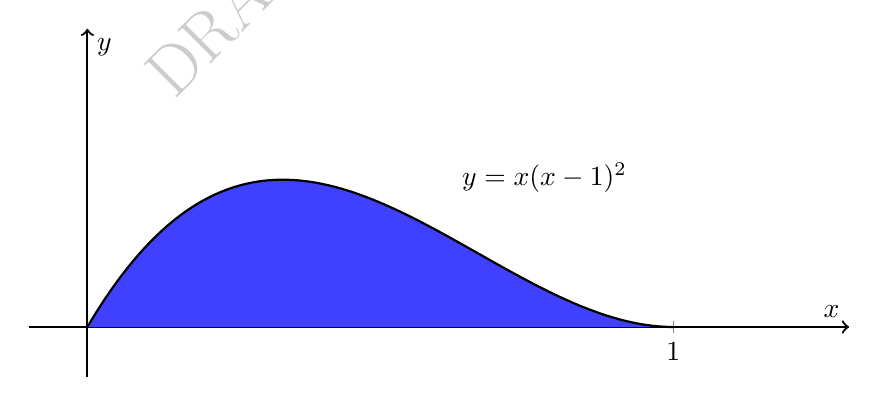
\begin{tikzpicture}
\begin{axis}[
    width=12cm,          % Makes the graph wider
    height=6cm,          % Controls vertical scaling
    axis lines=middle,
    axis line style={->,thick},
    xmin=-0.1, xmax=1.3,
    ymin=-0.05, ymax=0.3,
    xtick={0,1},
    xticklabels={0,1},
    ytick=\empty,
    xlabel={$x$},
    ylabel={$y$},
    enlargelimits=false,
    domain=0:1,
    samples=300,
    clip=false,
]

% Shaded area under the curve from 0 to 1
\addplot[draw=none, fill=blue!75] {x*(x-1)^2} \closedcycle;

% Curve y = x(x-1)^2
\addplot[thick, black] {x*(x-1)^2};

% Label on the curve
\node at (axis cs:0.78,0.15) {$y=x(x-1)^2$};

\end{axis}
\end{tikzpicture}
\end{center}


\subsection*{Solution}

\subsubsection*{Method 1: Conceptual reason washers are awkward (geometry of cross-sections)}

When rotating about the \(y\)-axis, the disk-washer method uses \emph{horizontal} slices (integrating with respect to \(y\)) and requires radii written as functions of \(y\):
\[
V=\pi\int_{y_{\min}}^{y_{\max}}\big(R(y)^2-r(y)^2\big)\,dy.
\]
Here the region is bounded by \(y=x(x-1)^2\), the \(x\)-axis, and \(0\le x\le 1\). The main issue is that
\[
y=f(x)=x(x-1)^2
\]
is \emph{not} one-to-one on \([0,1]\): it increases on \([0,\tfrac13]\) and decreases on \([\tfrac13,1]\). In particular,
\[
f'(x)=3x^2-4x+1=(3x-1)(x-1),
\]
so the maximum occurs at \(x=\tfrac13\), giving
\[
y_{\max}=f\!\left(\tfrac13\right)=\frac{4}{27}.
\]
For each \(y\) with \(0<y<\frac{4}{27}\), a horizontal line intersects the curve at \emph{two} \(x\)-values:
\[
x=x_L(y)\in\left(0,\tfrac13\right)\quad\text{and}\quad x=x_R(y)\in\left(\tfrac13,1\right).
\]
Thus a typical cross-section perpendicular to the \(y\)-axis becomes a \emph{washer} with
\[
R(y)=x_R(y),\qquad r(y)=x_L(y),
\]
and determining \(x_L(y)\) and \(x_R(y)\) requires solving the cubic equation \(x(x-1)^2=y\), i.e.
\[
x^3-2x^2+x-y=0,
\]
which is algebraically messy and would lead to a complicated setup (two branches \(x_L(y)\) and \(x_R(y)\)). This is why washers are awkward here.

\subsubsection*{Method 2: Cylindrical shells (standard setup about the \(y\)-axis)}

Using vertical shells (integrating with respect to \(x\)), a typical shell at position \(x\) has:
\begin{itemize}[leftmargin=*]
\item radius \(=x\),
\item circumference \(=2\pi x\),
\item height \(= (\text{top }y\text{-value at }x)-(\text{bottom }y\text{-value at }x)
= x(x-1)^2-0 = x(x-1)^2.\)
\end{itemize}
Hence the volume is
\[
V=2\pi\int_{0}^{1} x\cdot \big(x(x-1)^2\big)\,dx
=2\pi\int_{0}^{1} x^2(x-1)^2\,dx.
\]
Expand and integrate:
\[
x^2(x-1)^2=x^2(x^2-2x+1)=x^4-2x^3+x^2,
\]
so
\[
V=2\pi\int_{0}^{1}\left(x^4-2x^3+x^2\right)\,dx
=2\pi\left[\frac{x^5}{5}-\frac{2x^4}{4}+\frac{x^3}{3}\right]_{0}^{1}.
\]
Evaluate:
\[
V=2\pi\left(\frac15-\frac12+\frac13\right)
=2\pi\left(\frac{6-15+10}{30}\right)
=2\pi\cdot\frac{1}{30}
=\frac{\pi}{15}.
\]

\[
\boxed{V=\frac{\pi}{15}}
\]



\end{document}